\section{Lezione 12}%
\label{sub:Lezione 12}
\subsection{Simulazione del processo di Wiener in una doppia buca.}%
\label{sub:Simulazione dei camminatori.}
Riprendiamo l'ultimo argomento della lezione \ref{sub:Parte 2}, ovvero il calcolo del tempo di primo passaggio con un metodo più potente. \\
Prendiamo un sistema di camminatori che seguono la seguente SDE:
\[\begin{aligned}
    dx = & f(x) dt + \sqrt{\epsilon} dW = \\
    = & \left(x-x^3\right)dt + \sqrt{\epsilon} dW
.\end{aligned}\]
In cui $f(x)$ è la forza che sente il camminatore in un potenziale a doppia buca della forma:
\begin{figure}[H]
    \centering
    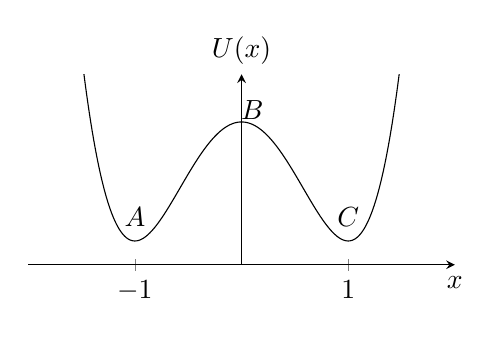
\begin{tikzpicture}
	\begin{axis}[
	    width=7cm,
	    height=4cm,
	    xmin= -2, xmax= 2,
	    ymin= 0, ymax = 0.4,
	    axis lines = middle,
	    x label style={at={(axis description cs:1,-0.01)},anchor=north},
	    y label style={at={(axis description cs:0.5,1)},anchor=south},
	    xlabel={$x$},
	    ylabel={$U(x)$ },
	    xtick={0, 1, -1},
	    xticklabels={$0$, $1$, $-1$},
	    ytick={0},
	    yticklabel={$0$},
	    ]
	    \addplot[domain=-3:3, samples=500]{-x^2/2*(1-x^2/2) + 0.3};
	    \node (C) [mark=dot] at (axis cs: 1, 0.1) {$C$};
	    \node (B) [mark=dot] at (axis cs: 0.1, 0.325) {$B$};
	    \node (A) [mark=dot] at (axis cs: -1, 0.1) {$A$};
	\end{axis}
    \end{tikzpicture}
    \caption{\scriptsize Potenziale in cui vivono i camminatori (l'integrale di $f$ con il segno invertito).}
    \label{fig:lore}
\end{figure}

\noindent
Ipotizziamo di inserire tutti i camminatori nel punto $A$, il sistema grazie al processo di Wiener $dW$ inizia a muoversi e può capitare che un camminatore riesca a raggiungere il punto $B$ cadendo poi nella buca con minimo in $C$. \\
Quello che vogliamo capire è se tutti i processi di Wiener possono permettere questo tipo di moto oppure se serve una configurazione particolare di $dW_n$ per raggiungere la buca $C$. Per capirlo operativamente si eseguono i seguenti passaggi:
\begin{itemize}
    \item Si simula il sistema ipotizzando $\sqrt{\epsilon} \ll f(x) \ \forall x$.
    \item ad evoluzione finita si considerano solo le traiettorie $x^{(j)}$ che hanno raggiunto $C$ al tempo $t^{(j)}$.
    \item Si trasla l'origine temporale di ogni traiettoria $x^{(j)}$ nell'istante in cui tale traiettoria ha raggiunto $C$.
    \item Si graficano tutte le traiettorie in un unico plot.
\end{itemize}
Effettuando una simulazione multipla seguendo questo procedimento si ottiene:
\begin{figure}[H]
    \centering
    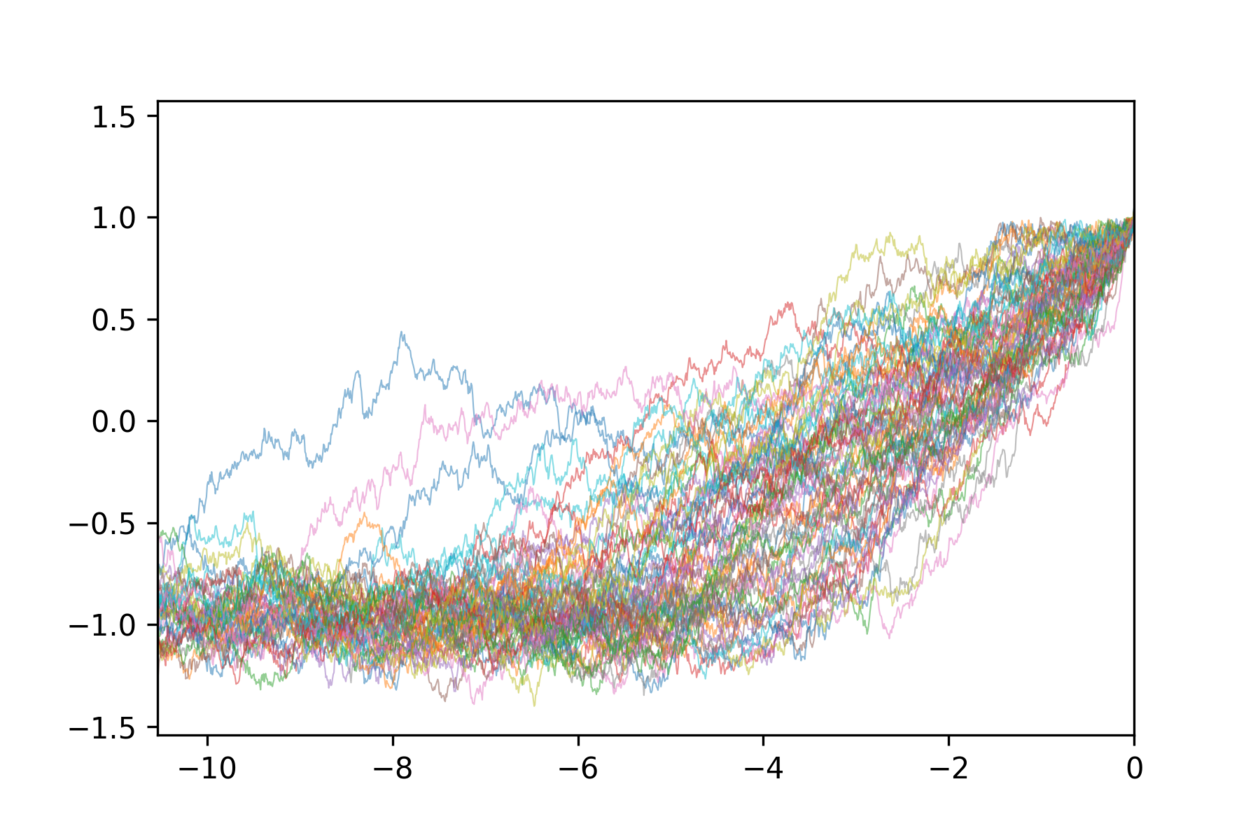
\includegraphics[width=0.5\textwidth]{figures/lez_12_walker_t_path.png}
    \caption{\scriptsize 70 camminatori che raggiungono il punto C.}
    \label{fig:figures-lez_12_walker_t_path-png}
\end{figure}
\noindent 
Si nota come tutte le traiettorie sembrino seguire un percorso specifico, incanalandosi in una specie di tubo di flusso per arrivare in $x=1$. \\
Questa cosa appare evidente se andiamo a vedere la densità dei punti in cui nei quali è passato il camminatore:
\begin{figure}[H]
    \centering
    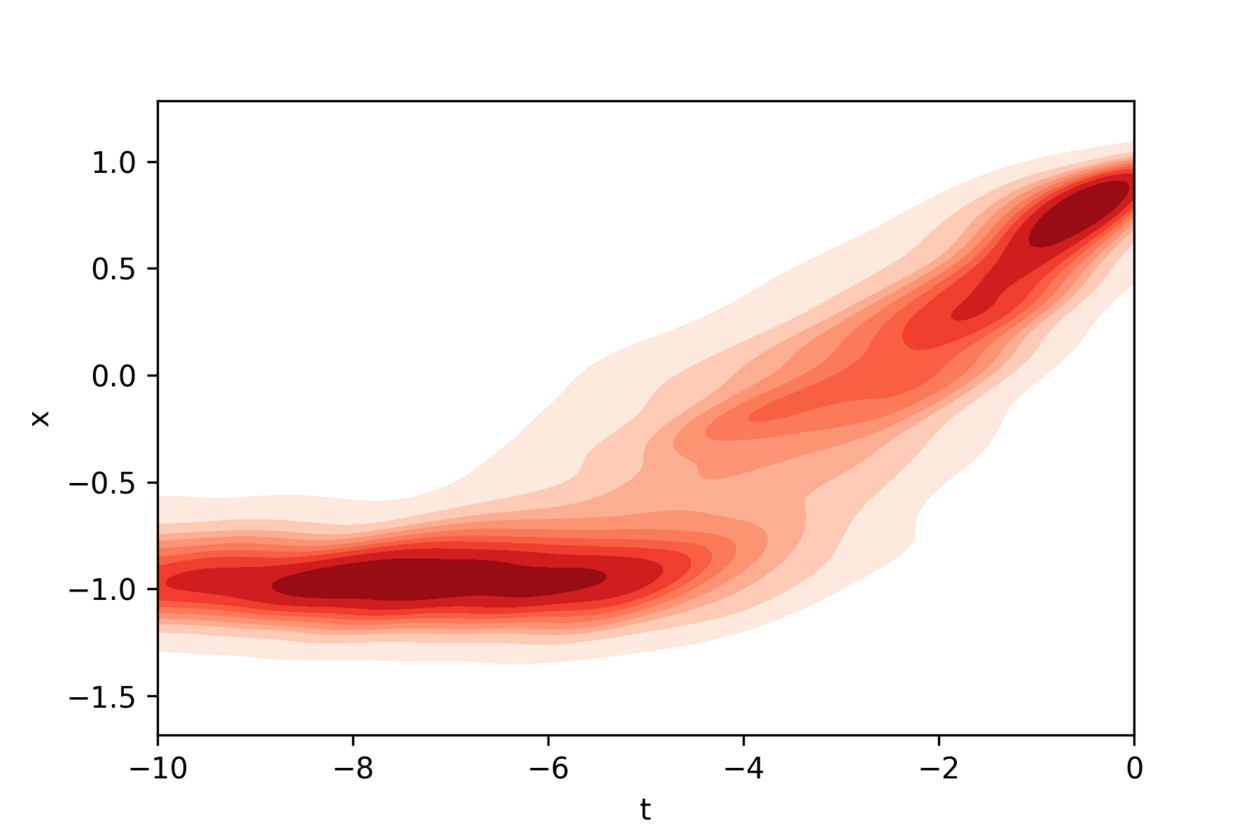
\includegraphics[width=0.5\textwidth]{figures/lez_12_walker_t.png}
    \caption{\scriptsize Densità dei camminatori che riescono a fare il salto nel tempo, si nota che si addensano attorno ad un tubo di flusso}
    \label{fig:figures-lez_12_walker_t-png-}
\end{figure}
\noindent 
Una cosa molto interessante da notare è la scala temporale, se mediamente un camminatore impiega un tempo di $100$ digit per scappare dalla buca $A$ restringendoci ai soli camminatori che riescono nell'impresa questo tempo risulta essere inferiore a $8$ digit. \\
Questo significa che la sequenza di $dW_n$ che permette il passaggio è molto improbabile, infatti deve essere tale da spingere il camminatore oltre una barriera!\\
Si possono prendere tutte le sequenze di $dW$ che hanno permesso ai $70$ camminatori di attraversare la barriera e valutarne la densità in $x$. Il seguente grafico mostra un istogramma bidimensionale ('countour plot') del rumore in funzione di $x$:
\begin{figure}[H]
    \centering
    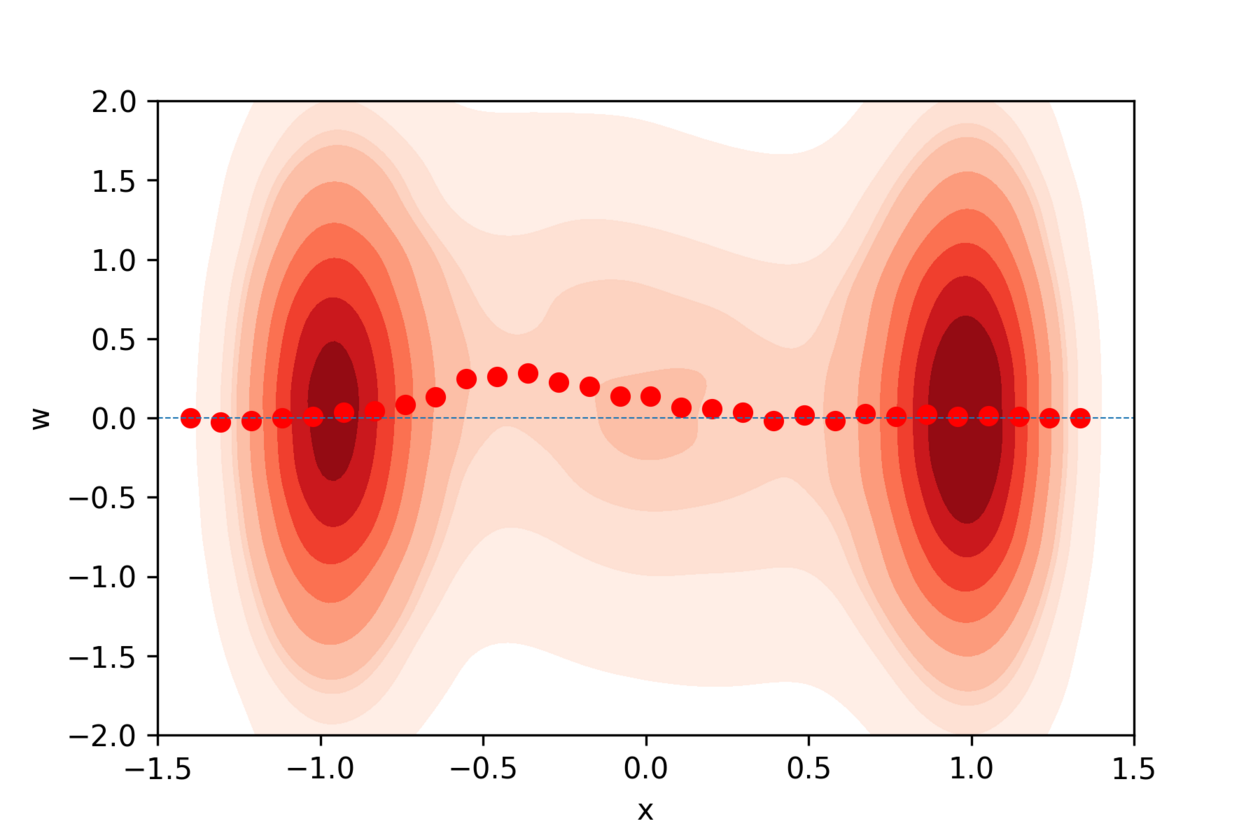
\includegraphics[width=0.5\textwidth]{figures/lez_12_dist.png}
    \caption{\scriptsize Distribuzione del processo stocastico per i camminatori che riescono a fare il salto, notiamo che la media del processo (curva arancione) deve essere diversa da zero.}
    \label{fig:figures-lez_12_dist-png}
\end{figure}
\noindent
Possiamo notare il fatto che per ottenere una sequenza giusta il rumore debba essere diverso da zero (e positivo) lungo la salita del potenziale. \\
Superata la barriera allora il rumore può gradualmente rilassare: la fatica ormai è fatta. 

\subsection{Hamiltoniana per il MFPT}%
\label{sub:Hamiltoniana per il MFPT}
Riprendiamo l'equazione per il processo in forma discretizzata:
\[
    x_{n+1} = x_n + f(x_n) \Delta t + \sigma \Delta\omega_n = F(x_n) + \xi_n
.\] 
\[
    \left<\xi_n\xi_m\right> = \epsilon\Delta_{nm}
.\] 
Consideriamo sempre l'intervallo $(a,b)$ come sopra. Abbiamo visto che la probabilità di andare da $a$ a $b$ 
\[
    P\left(x_b,t|x_a,0\right)
.\] 
è legata alla probabilità di una "corretta" fluttuazione di $\xi$. \\
Supponiamo di discretizzare il tempo con un passo $\Delta t$:
\[
    t_{i+1} = t_i + \Delta t 	\quad \forall i
.\] 
La probabilità di arrivare in $b$ può essere scritta come una catena di propagatori:
\[\begin{aligned}
    P\left(x_b,t|x_a,t_0\right)=&P\left(x_1,t_1|x_a,t_0\right)\cdot P\left(x_2,t_2|x_1,t_1\right)\cdot \ldots \\
				&\ldots \cdot P\left(x_b,t_b|x_{n-1},t_{n-1}\right)
.\end{aligned}\]
Dove si sfrutta in questo passaggio il fatto che il sistema è markoviano (quindi è lecito scrivere la probabilità composta in questo modo).\\
Notiamo che la probabilità di fare il salto dalla posizione $x_{i}$ a quella $x_{i+1}$ deve essere legato alla probabilità di ottenere il "giusto" $\xi_i$  del processo di Wiener:
\[
    P\left(x_{i+1}, t_{i+1}|x_i,t_i\right) \sim P(\xi_i) 
.\] 
\[
    \text{Con } \xi_i: \quad x_{i+1} = F(x_i) + \xi_i
.\] 
Sia $\gamma$ una fluttuazione ottimale che permette il passaggio da $a$ a $b$.
\[
	\gamma \to \left[\zeta_1, \ldots, \zeta_n\right]
.\] 
La probabilità che tale fluttuazione avvenga avrà la forma:
\[
    P(\gamma) \sim \exp\left(-\frac{S\left[x_1,\ldots,x_n\right]}{\epsilon}\right)
.\] 
\[
    S = \frac{1}{2}\sum_{}^{} \zeta^2_i
.\] 
Quindi il tempo di primo passaggio può essere ricavato dal fatto che:
\[
    P\left(x_n,t_n = T|x_0,t_0\right) \sim k \exp\left(-\frac{S_{\text{min}}}{\epsilon}\right)
.\] 
Quello che cerchiamo è il minimo dell'azione $S$: $\overline{S}$, ovvero la sequenza $\gamma$ che massimizza la probabilità di fare il salto $a\to b$.\\
Per risolvere il problema di minimo possiamo utilizzare un set di moltiplicatori di Lagrange $\lambda_i$.
\[
    \overline{S} = \frac{1}{2}\sum_{i}^{} \zeta^2_i + \lambda_i \left[x_{i+1}-F(x_i)- \zeta_i\right]
.\] 
Risolvendo il problema dei moltiplicatori si ottiene:
\[\begin{aligned}
    &1. \quad x_{n+1} = F(x_n) + \lambda_n\\
    &2. \quad \lambda_{n+1}=\left[\left.\frac{\partial F}{\partial x_i} \right|_{i = n+1}\right]^{-1}\lambda_n
.\end{aligned}\]
Passiamo a tempi continui, chiamiamo $\Delta t = h$, dalla prima equazione si ottiene che
\footnote{Non mi torna l'$h$, mi pare sparita\ldots}
:
\[
    x_{n+1} = x_n + h f(x_n) + \lambda_n \implies  \dot{x} = f + \lambda
.\] 
La seconda equazione può essere manipolata considerando la definizione di $F$:
\[
    F(x_n) = x_n+hf(x_n) \quad \implies  \quad  \frac{\partial F}{\partial x} = 1+hf'
.\] 
Sostituendo questa nella (2.) e sommando e sottraendo $\lambda_n$ si arriva a:
\[
    \dot{\lambda} =  - f'\lambda
.\] 
Ci siamo ricondotti a due equazioni da integrare con le opportune condizioni al contorno:
\begin{redbox}{Equazioni di Hamilton per il sistema}
\[
    \begin{cases}
	\dot{x} = f(x) + \lambda\\
	\dot{\lambda } = - f'(x) \lambda
    \end{cases}
.\]     
\end{redbox}
\noindent
l'Hamiltoniana che corrisponde a queste equazioni è della forma:
\[
    \lambda  \to p \quad \implies  \quad H = \frac{p^2}{2} + pf
.\] 
Infatti vale che:
\[
    \begin{cases}
	\dot{x} = \left[x,H\right]\\
	\dot{p} = \left[p,H\right]
    \end{cases}
.\] 
Le condizioni al contorno che possiamo usare per risolvere sono 
\[
    x(t=0) = a; \quad x(t = t_n) = b
.\] 
Il problema può essere risolto con il calcolo della azione, sappiamo che l'azione di un sistema è legata alla lagrangiana dalla seguente:
\[
    \dot{S} = \mathcal{L} = \frac{\partial H}{\partial P} P - H
.\] 
Quindi operativamente basta integrare la lagrangiana per ottenere la $S$, minimizzarla per avere la $P$, visto che $P$ è proporzionale al tempo di primo passaggio $T$. 
\subsubsection{Applicazione del metodo ad un potenziale $U(x)$}%
\label{subsub:Applicazione del metodo ad un potenziale $U(x)$}
Prendiamo l'equazione per l'incremento di $x$:
\[
    dx = - U' dt + \sqrt{\epsilon} d\omega
.\] 
In cui si ha che, come già accennato $-U' = f$.\\
Risolviamo le equazioni di Hamilton:
\[
    \begin{cases}
	\dot{x} = -U' + p\\
	\dot{p} = U''p
    \end{cases}
.\] 

